\subsection{Forward kinematic equations of Fanuc 210F}

\subsubsection{Joint and link numbering in Fanuc 210F}
The numbering scheme presented in \fullref{sec:NumJointLink} can be applied to the Fanuc 210F (see \ref{fig:LinksANDJoints210F}) 


\begin{figure}[H]
	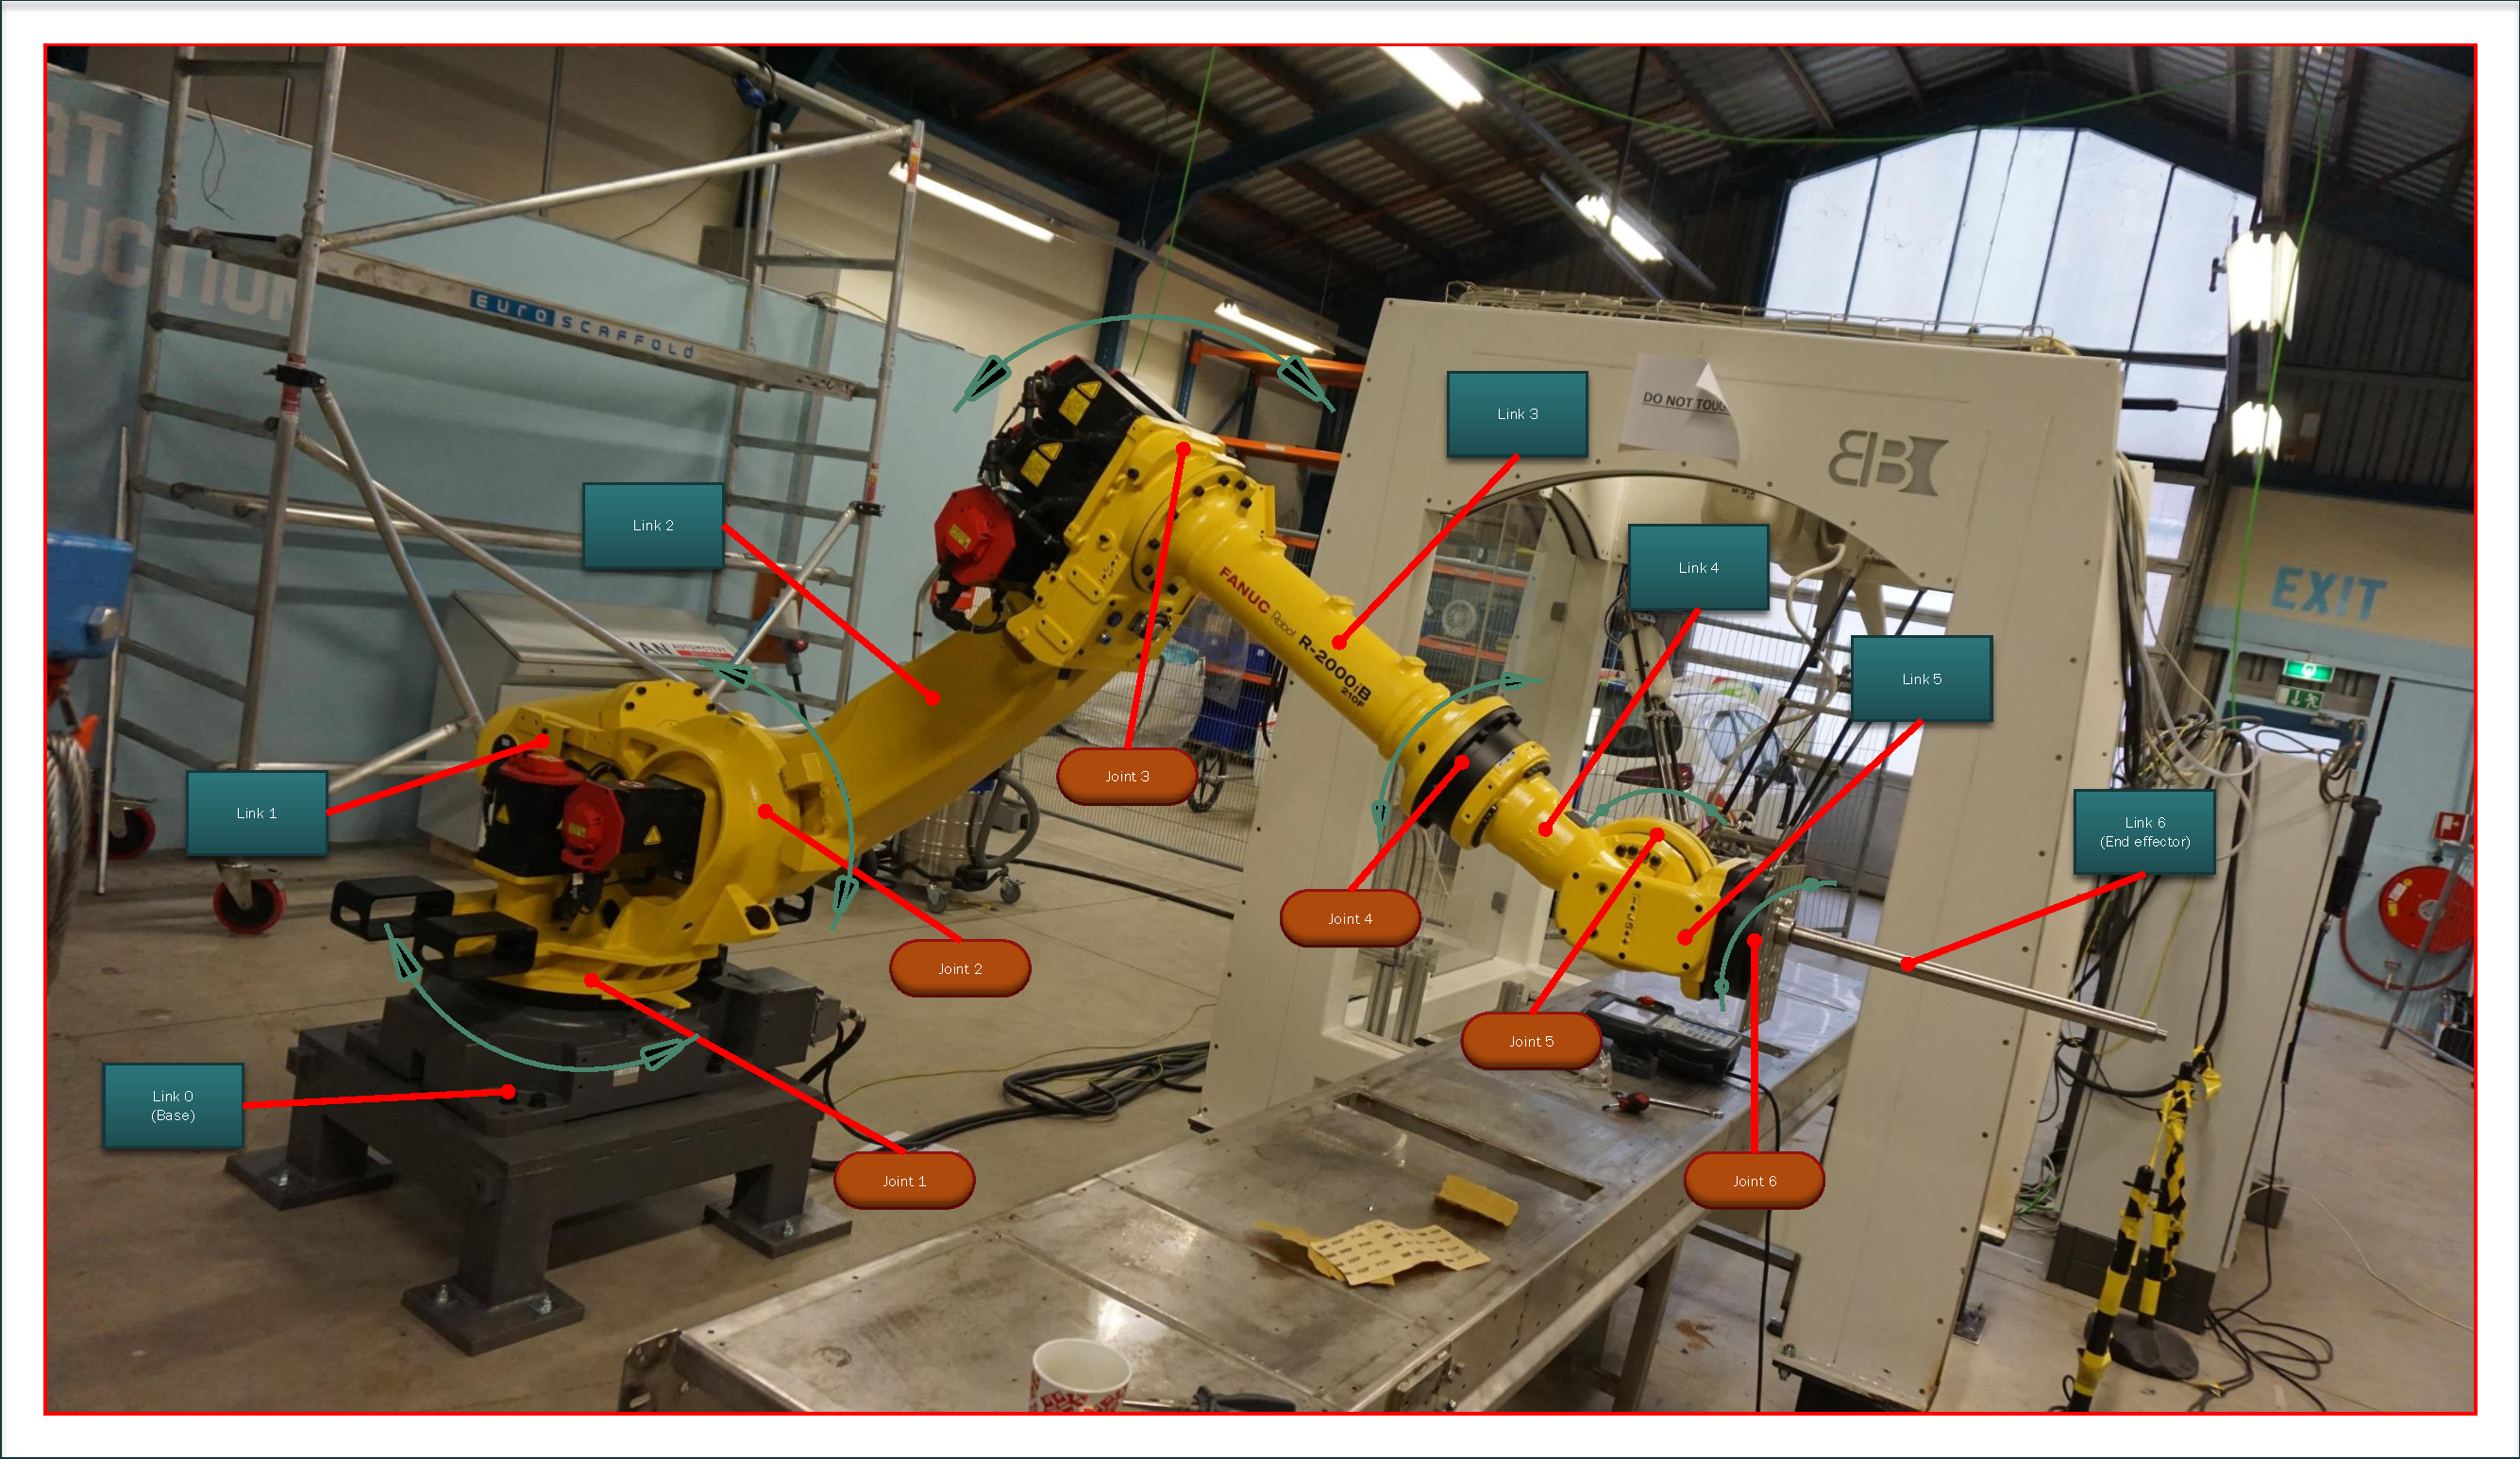
\includegraphics[
	width=1\linewidth,
	center,
	keepaspectratio,
	]{linksANDjoints/linksAndJoints}
	\caption{Links (turquoise) and joints (orange) in the FANUC 210F}
	\label{fig:LinksANDJoints210F}
\end{figure}

\paragraph{$z_i$ axes in Fanuc 210F}
As described in \fullref{par:z_iAxesAssign}, the $z_i$ axes can be attached to the Fanuc 210F (see figure \ref{fig:zi_Axes}).


\begin{figure}[H]
	\includegraphics[
	width=1\linewidth,
	center,
	keepaspectratio,
	]{coordinateFrames/z_axes}
	\caption{$z_i$ axes on the Fanuc 210F with the direction of positive rotation (orange)}
	\label{fig:zi_Axes}
\end{figure}


The positive direction of the triples $z_1$, $z_2$, $z_4$ and $z_0$, $z_3$, $z_5$, was chosen to make sure, the x-axis would always have the same direction for parallel joints. 

\subsubsection{local coordinate reference frames on the Fanuc 210F}

As described in \fullref{sec:localRefFrame}, the local coordinate reference frames can also be attached to the Fanuc 210F as seen in figure \ref{fig:RefFrame}. 

\begin{figure}[h]
	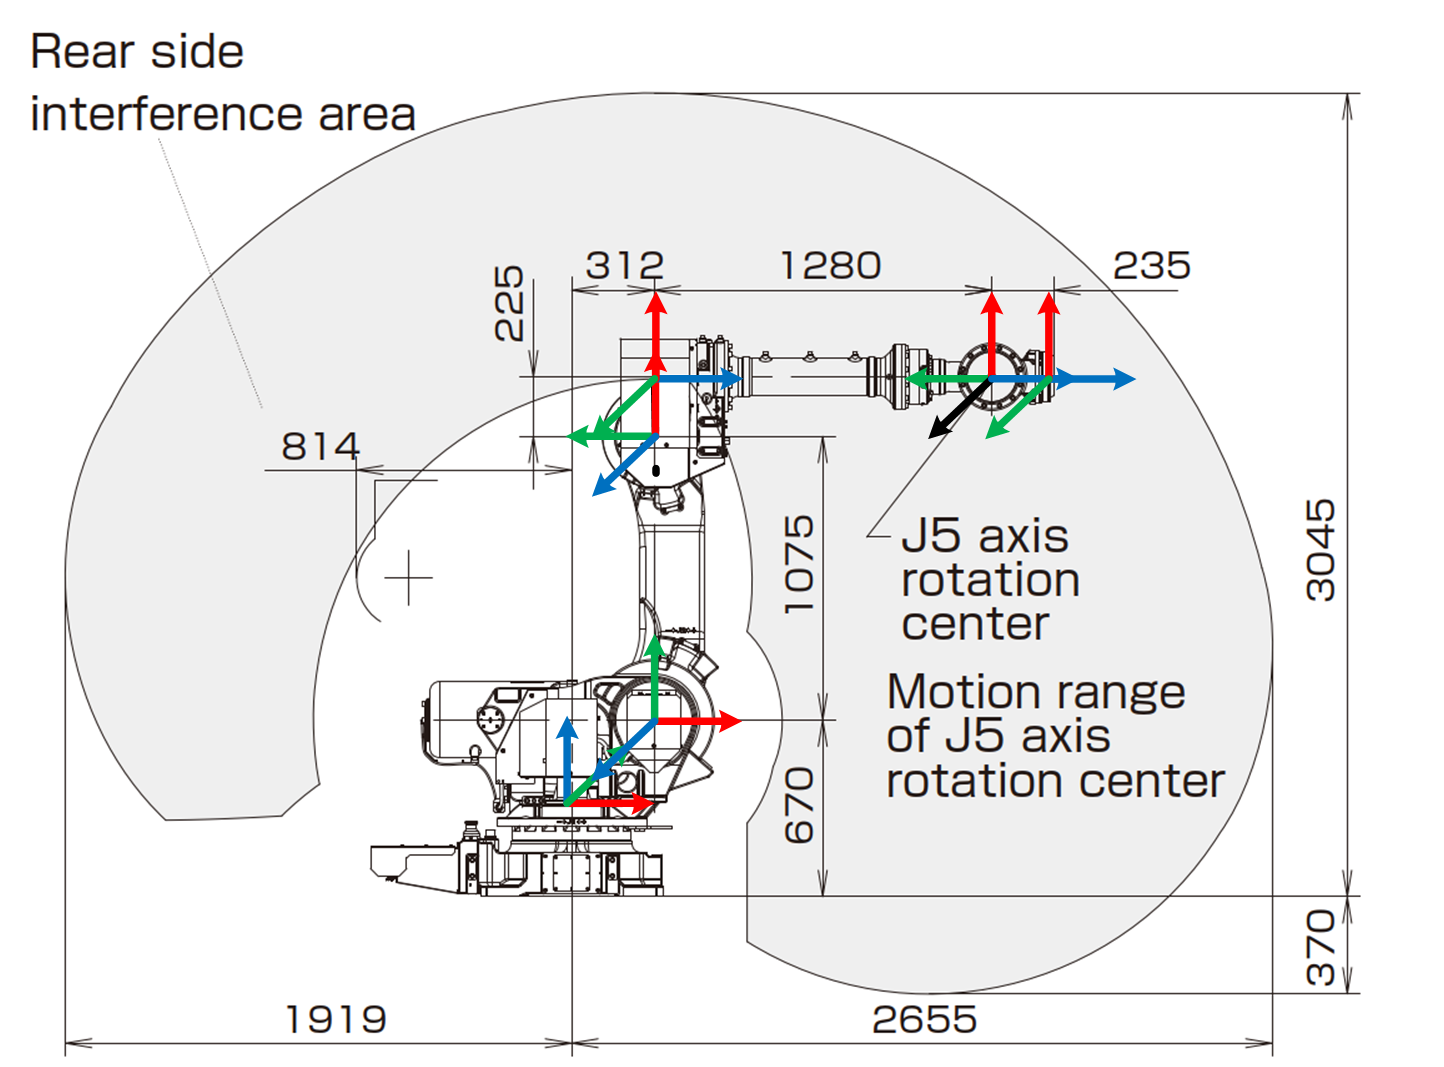
\includegraphics[
	width=1\linewidth,
	center,
	keepaspectratio,
	]{coordinateFrames/CoordinateFramesRobotStandardPose}
	\caption{Coordinate reference frames for Fanuc 210F in standard (Normal) pose}
	\label{fig:RefFrame}
\end{figure}


\paragraph{Abstract view of coordinate frames}
For a better overview, the drawing of the robot can be removed, which reveals the pure coordinate frames. Here it can be described, in which relation the coordinate frames stand in relation to each other.

\begin{figure}[h]
	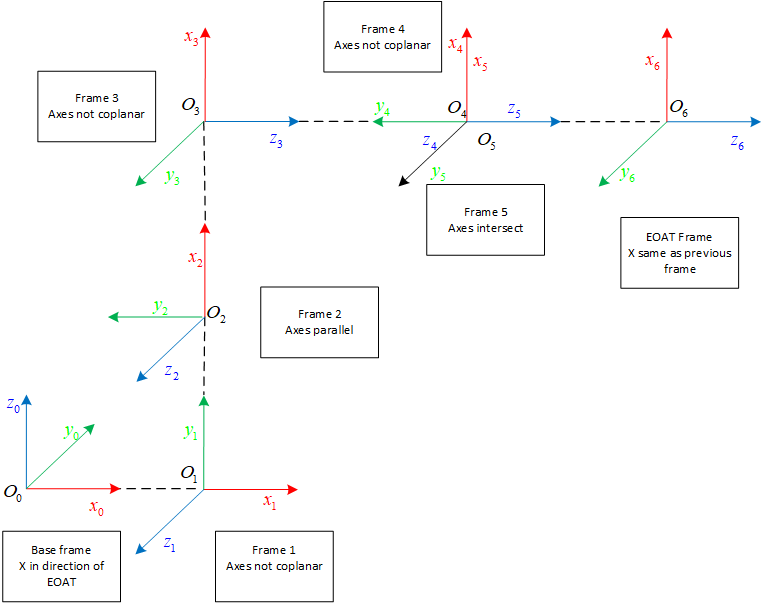
\includegraphics[
	width=1\linewidth,
	center,
	keepaspectratio,
	]{coordinateFrames/CoordinateFrames}
	\caption{Coordinate reference frames for Fanuc 210F}
	\label{fig:RefFrameAbstract}
\end{figure}

\paragraph{frame 0 (Base)}
The frame mapping starts with the base frame. For the base frame the z-axis is given through joint $j_1$. Origin of frame 0 is put into joint 1.
The x-axis is chosen to point in direction of of the \ac{EOAT} in standard pose. For standard pose see \ref{fig:RefFrame}.
This pose will also be chosen for alignment of all distal frames.

%\begin{figure}[h]
%	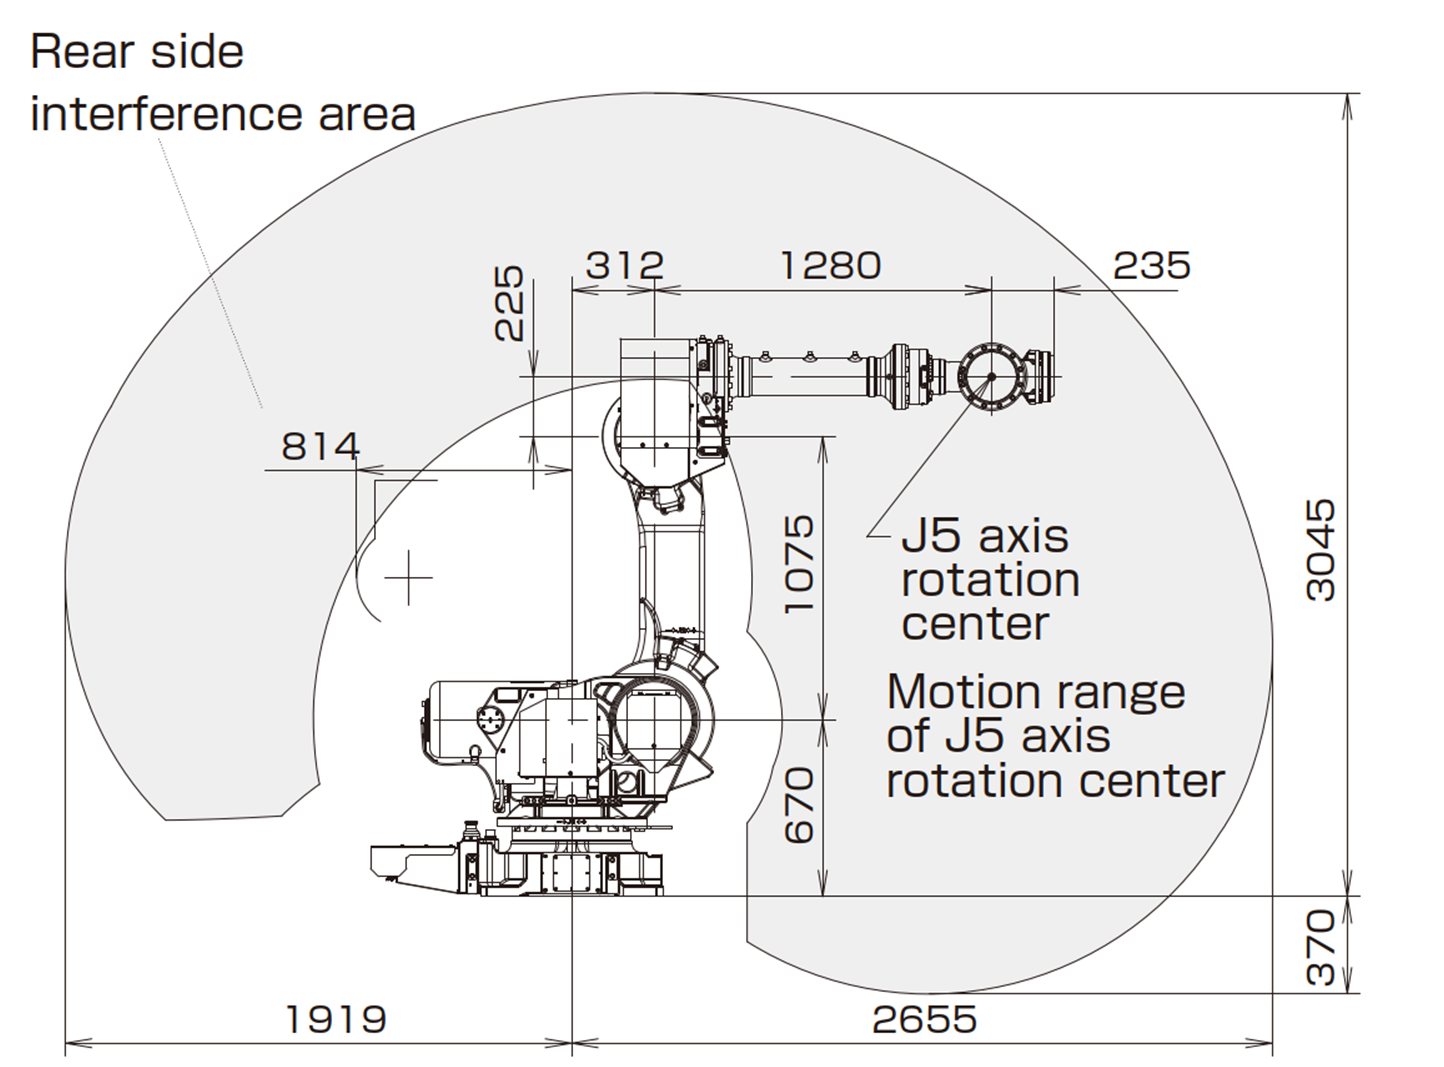
\includegraphics[
%	width=1\linewidth,
%	center,
%	keepaspectratio,
%	]{coordinateFrames/standardPose}
%	\caption{Standard pose of the robot}
%	\label{fig:StandardPose}
%\end{figure}

\paragraph{frame 1}
For frame 1, the z-axes are not coplanar. 
Because of that, the  $z_0$-axis is extended until a common normal can be found that intersects with $z_i$ to define the origin $O_1$.
$x_1$ departs from $O_1$ along the common normal.
$y_1$ is added according to the right hand rule.

\paragraph{frame 2}
As seen, in image \ref{fig:zi_Axes}, axes $z_2$ and $z_1$ are parallel. $O_2$ can be found at the intersection of the normal through $O_1$ with $z_2$. $x_2$ follows the common normal with joint 4.
$y_2$ is added according to the right hand rule.

\paragraph{frame 3}
Joint 3 and joint 4 are not exactly aligned (see image \ref{fig:RefFrame}), which prevents the z-axes to intersect. That's why axes $z_3$ and $z_2$ are not coplanar. 
$z_3$ runs parallel through the link 3, due to the orientation of the rotational axis.
As the common normal between $z_3$ and $z_2$ defines $x_3$, which in turn gives $O_3$, the origin can be found far away from the physical position of the joint.
$y_3$ is added according to the right hand rule.

\paragraph{frame 4}
Joint 5 lies in line with joint 4.
As $z_3$ follows this line, the axes  $z_4$ and $z_3$ intersect in the center of joint 5, which gives $O_4$. 
$x_4$ leaves the plane spanned by  $z_4$ and $z_3$ perpendicular.
The positive direction of $x_4$ is chosen to be similar as in frame 3 for simplicity.
$y_4$ is added according to the right hand rule and points in direction of frame 3.

\paragraph{frame 5}
As $z_5$ lies  in line with $O_4$, the axes  $z_5$ and $z_4$ intersect in $O_4$ which puts $O_5$ at the same position as $O_4$.
$x_5$ leaves the plane spanned by  $z_5$ and $z_4$ perpendicular.
The positive direction of $x_5$ is chosen to be similar as in frame 4 for simplicity, which puts $x_5$ and $x_4$ on top of each other. 
$y_5$ is added according to the right hand rule and as $z_5$ is turned 90 degrees relative to $z_4$ around $x_{4,5}$, $y_5$ is turned 90 degrees relative to $z_4$ around $x_{4,5}$ as well.

\paragraph{frame 6 (EOAT)}
$z_6$ lies in line with $z_5$ and is consequently parallel.
as there are no distal joints, to reference $x_6$, it can be chosen arbitrarily. 
For simplicity, it is chosen to be similar as in frame 5. 
$y_6$ is added according to the right hand rule.


\subsubsection{Establishing \ac{DH} parameters on the Fanuc 210F}

As described in \fullref{sec:DHparPerLink}, the \ac{DH}-Parameters can also be determined for the Fanuc 210F.
These parameters can be found with the help of the assigned coordinate frames as seen in figure \ref{fig:DH_Parameters_Fanuc210F}. For simplicity, only non-zero DH-parameters are shown in this figure.

\begin{figure}[H]
	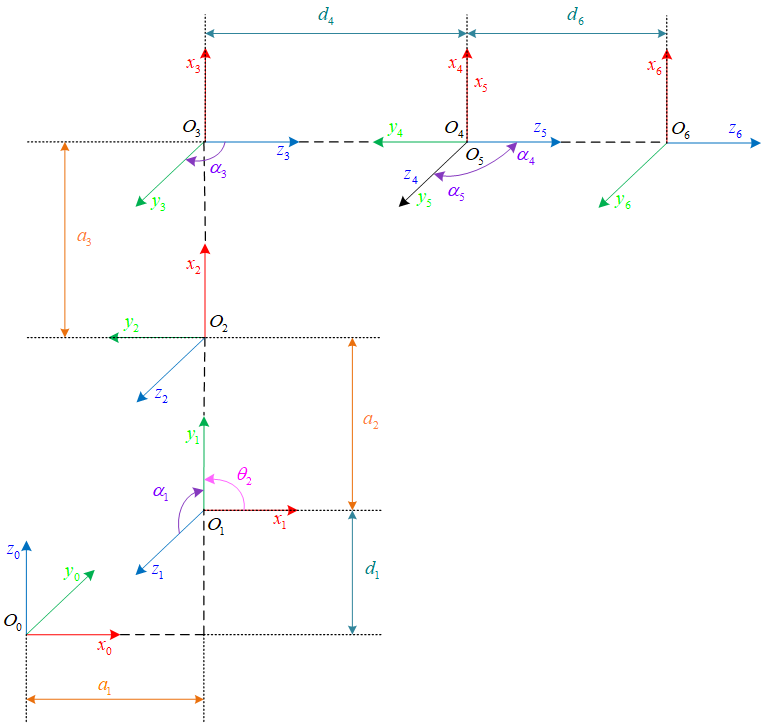
\includegraphics[
	width=1\linewidth,
	center,
	keepaspectratio,
	]{coordinateFrames/DH_Parameters_assignment}
	\caption{Assignment of DH-Parameters on the Fanuc 210F}
	\label{fig:DH_Parameters_Fanuc210F}
\end{figure}


To wrap this up, a summary of the D-H parameters for each link as follows from figure \ref{fig:DH_Parameters_Fanuc210F} can be found in table \ref{table:DH-Parameter}


%Generate tables easily with: % https://www.tablesgenerator.com/

\begin{table}[H]
	\centering
	\begin{tabular*}{0.5\textwidth}{|l||@{\extracolsep{\fill}}l|l|l|l|}
		\hline
		Link & \multicolumn{1}{l|}{$\theta_i$} & \multicolumn{1}{l|}{$d_i$} & \multicolumn{1}{l|}{$a_i$} & \multicolumn{1}{l|}{$\alpha_i$} \\ \hline\hline
		1 & $\theta_1$ & $d_1$ & $a_1$ & $\alpha_1$\\ \cline{1-5}
		2 & $\theta_2$ & 0     & $a_2$ & 0         \\ \cline{1-5}
		3 & $\theta_3$ & 0     & $a_3$ & $\alpha_3$\\ \cline{1-5}
		4 & $\theta_4$ & $d_4$ & 0     & $\alpha_4$\\ \cline{1-5}
		5 & $\theta_5$ & 0     & 0     & $\alpha_5$\\ \cline{1-5}
		6 & $\theta_6$ & $d_6$ & 0     & 0         \\ \cline{1-5}
		%\hline
	\end{tabular*}
	\caption{Denavit Hartenberg Parameters for Fanuc 210F}
	\label{table:DH-Parameter}
\end{table}


\paragraph{numeric values of DH-Parameters}

As can be seen from table \ref{table:DH-Parameter}, many \ac{DH}-parameters are zero due to a good choice of pose and coordinate frames. 
All angles are plus or minus 90°.

Most of the frames have translational transformations in either $a_i$ or $d_i$ direction with link 1 and 5 being the exception.
By lifting the base frame out of the joint, parameter $d_1$ could be set to zero as well. For better understanding, the origin of the frame was originally kept inside the joint.
Frame 5 shares the origin with frame 4, not requiring any translational movement.
Most of the frames are also rotated by 90 degree around the x-axis with link 2 and 6 being the exception. Frame 6 was chosen with the same orientation as frame 5. Frame 2 has the same x-axis orientation as link 1 because joints two and three are parallel. There is just a rotational transformation around the z-axis of 90°. This is only due to the standard pose of the robot, as theta is a variable.
For all coordinate frames theta is a variable, as all joints are revolute and none is translational. 

Besides the angle values for $\alpha_i$ which were easy to determine from the graphical interpretation in figure \ref{fig:DH_Parameters_Fanuc210F}, following numeric values need to be determined through measurements or CAD-Drawings:
$d_1$, $d_4$, $d_6$ and \\
$a_1$, $a_2$, $a_3$. 

A great help to determine these values is fig \ref{fig:RefFrame}. This technical drawing was obtained from the datasheet for all Fanuc R-2000iB series robots. 
With this drawing, following \ac{DH}-parametes can be obtained:

\begin{itemize}\label{item:DH-LinparamValues}
	\item[$a_1$=] 312 [\textit{mm}]
	\item[$a_2$=] 1075 [\textit{mm}]
	\item[$a_3$=] 225 [\textit{mm}]
	\item[$d_4$=] 1280 [\textit{mm}]
	\item[$d_6$=] 235 [\textit{mm}]
\end{itemize}

The parameter $d_1$ cannot be determined from this drawing. It can either be measured on the actual robot, or defined as zero, as frame zero can be freely moved along the z-axis. A value of zero would put the origin of the base frame on the same height as frame 1, simplifying subsequent steps. 
It must be clear though, that all referencing in the forward and backward kinematics will be relative to this point. 
A change of this point of reference can be added later simply by adding another transformation matrix for translational movement along the z-axis as presented by Richard P. Paul \cite{Paul1981RobotM}.\\
\\
This results in a table of numeric DH-parameters as seen in \ref{table:DH-Parameter_num}. The transformation $^{i-1}T_i$ depends only on a single variable $\theta_i$ as all of the other quantities stay constant, and all joints are revolute.

\begin{table}[H]
	\centering
	\begin{tabular*}{0.5\textwidth}{|l||@{\extracolsep{\fill}}l|l|l|l|}
		\hline
		Link & \multicolumn{1}{l|}{$\theta_i$} & \multicolumn{1}{l|}{$d_i$} & \multicolumn{1}{l|}{$a_i$} & \multicolumn{1}{l|}{$\alpha_i$} \\ \hline\hline
		1 & $\theta_1$ & 0     & 312   & $\pi/2$  \\ \cline{1-5}
		2 & $\theta_2$ & 0     & 1075  & 0        \\ \cline{1-5}
		3 & $\theta_3$ & 0     & 225   & $\pi/2$  \\ \cline{1-5}
		4 & $\theta_4$ & 1280  & 0     & $-\pi/2$ \\ \cline{1-5}
		5 & $\theta_5$ & 0     & 0     & $\pi/2$  \\ \cline{1-5}
		6 & $\theta_6$ & 235   & 0     & 0        \\ \cline{1-5}
		%\hline
	\end{tabular*}
	\caption{Numeric values of Denavit Hartenberg Parameters for Fanuc 210F}
	\label{table:DH-Parameter_num}
\end{table}


\subsubsection{Calculate homogeneous transformation matrices}

For further details on how to set up $R_z(\theta_i), T_z(d_i), T_x(a_i) and R_x(\alpha_i)$ and form the transformation matrix in equation \ref{eq:TransformationMarix} see chapter one "HOMOGENEOUS TRANSFORMATIONS" in "Robot manipulators: mathematics, programming, 
and control: the computer control of robot manipulators" \cite{Paul1981RobotM}. The basic techniques for setting up the translation and rotation matrices as well as how to combine them are described in that chapter .




\subsubsection{Forward Kinematic Equations on the 210F}
As shown in fig.\ref{fig:zi_Axes}, the Fanuc 210F is a 6-\ac{DOF} robotic arm with n=six revolute joints in series. 
Their orientation can be expressed in short form with 
\begin{equation}
(R\perp R\parallel R\perp R\perp R\perp R )
\end{equation}

With this, the complete transformation matrix can be derived in the form as described in \ref{ForKinEq}:

%\begin{equation}
\begin{multline}\label{eq:TransformMatrices_0-6}
	^0T_6=\\
	\begin{bmatrix}
\cos\theta_1 & -\sin\theta_1  \cos\alpha_1 & \sin\theta_1  \sin\alpha_1 & a_1  \cos\theta_1 \\
\sin\theta_1 & \cos\theta_1  \cos\alpha_1 & -\cos\theta_1  \sin\alpha_1 & a_1  \sin\theta_1 \\
0 & \sin\alpha_1 & \cos\alpha_1 & d_1 \\
0 & 0 & 0 & 1 \\
\end{bmatrix}
  \\
\begin{bmatrix}
\cos\theta_2 & -\sin\theta_2  \cos\alpha_2 & \sin\theta_2  \sin\alpha_2 & a_2  \cos\theta_2 \\
\sin\theta_2 & \cos\theta_2  \cos\alpha_2 & -\cos\theta_2  \sin\alpha_2 & a_2  \sin\theta_2 \\
0 & \sin\alpha_2 & \cos\alpha_2 & d_2 \\
0 & 0 & 0 & 1 \\
\end{bmatrix}
  \\
\begin{bmatrix}
\cos\theta_3 & -\sin\theta_3  \cos\alpha_3 & \sin\theta_3  \sin\alpha_3 & a_3  \cos\theta_3 \\
\sin\theta_3 & \cos\theta_3  \cos\alpha_3 & -\cos\theta_3  \sin\alpha_3 & a_3  \sin\theta_3 \\
0 & \sin\alpha_3 & \cos\alpha_3 & d_3 \\
0 & 0 & 0 & 1 \\
\end{bmatrix}
  \\
\begin{bmatrix}
\cos\theta_4 & -\sin\theta_4  \cos\alpha_4 & \sin\theta_4  \sin\alpha_4 & a_4  \cos\theta_4 \\
\sin\theta_4 & \cos\theta_4  \cos\alpha_4 & -\cos\theta_4  \sin\alpha_4 & a_4  \sin\theta_4 \\
0 & \sin\alpha_4 & \cos\alpha_4 & d_4 \\
0 & 0 & 0 & 1 \\
\end{bmatrix}
  \\
\begin{bmatrix}
\cos\theta_5 & -\sin\theta_5  \cos\alpha_5 & \sin\theta_5  \sin\alpha_5 & a_5  \cos\theta_5 \\
\sin\theta_5 & \cos\theta_5  \cos\alpha_5 & -\cos\theta_5  \sin\alpha_5 & a_5  \sin\theta_5 \\
0 & \sin\alpha_5 & \cos\alpha_5 & d_5 \\
0 & 0 & 0 & 1 \\
\end{bmatrix}
  \\
\begin{bmatrix}
\cos\theta_6 & -\sin\theta_6  \cos\alpha_6 & \sin\theta_6  \sin\alpha_6 & a_6  \cos\theta_6 \\
\sin\theta_6 & \cos\theta_6  \cos\alpha_6 & -\cos\theta_6  \sin\alpha_6 & a_6  \sin\theta_6 \\
0 & \sin\alpha_6 & \cos\alpha_6 & d_6 \\
0 & 0 & 0 & 1 \\
\end{bmatrix}
\phantom{  }\\
\end{multline}
%\end{equation}

This set of matrices can be filled with the numerical values from table \ref{table:DH-Parameter_num}:

%\begin{equation}
\begin{multline}
^0T_6=\\
\begin{bmatrix}
\cos\theta_1 & -\sin\theta_1*\cos(\pi/2) & \sin\theta_1*\sin(\pi/2) & 312*\cos\theta_1 \\
\sin\theta_1 & \cos\theta_1*\cos(\pi/2) & -\cos\theta_1*\sin(\pi/2) & 312*\sin\theta_1 \\
0 & \sin(\pi/2) & \cos(\pi/2) & 0 \\
0 & 0 & 0 & 1 \\
\end{bmatrix}
*\\
\begin{bmatrix}
\cos\theta_2 & -\sin\theta_2*\cos(0) & \sin\theta_2*\sin(0) & 1075*\cos\theta_2 \\
\sin\theta_2 & \cos\theta_2*\cos(0) & -\cos\theta_2*\sin(0) & 1075*\sin\theta_2 \\
0 & \sin(0) & \cos(0) & 0 \\
0 & 0 & 0 & 1 \\
\end{bmatrix}
*\\
\begin{bmatrix}
\cos\theta_3 & -\sin\theta_3*\cos(\pi/2) & \sin\theta_3*\sin(\pi/2) & 225*\cos\theta_3 \\
\sin\theta_3 & \cos\theta_3*\cos(\pi/2) & -\cos\theta_3*\sin(\pi/2) & 225*\sin\theta_3 \\
0 & \sin(\pi/2) & \cos(\pi/2) & 0 \\
0 & 0 & 0 & 1 \\
\end{bmatrix}
*\\
\begin{bmatrix}
\cos\theta_4 & -\sin\theta_4*\cos(-\pi/2) & \sin\theta_4*\sin(-\pi/2) & 0*\cos\theta_4 \\
\sin\theta_4 & \cos\theta_4*\cos(-\pi/2) & -\cos\theta_4*\sin(-\pi/2) & 0*\sin\theta_4 \\
0 & \sin(-\pi/2) & \cos(-\pi/2) & 1280 \\
0 & 0 & 0 & 1 \\
\end{bmatrix}
*\\
\begin{bmatrix}
\cos\theta_5 & -\sin\theta_5*\cos(\pi/2) & \sin\theta_5*\sin(\pi/2) & 0*\cos\theta_5 \\
\sin\theta_5 & \cos\theta_5*\cos(\pi/2) & -\cos\theta_5*\sin(\pi/2) & 0*\sin\theta_5 \\
0 & \sin(\pi/2) & \cos(\pi/2) & 0 \\
0 & 0 & 0 & 1 \\
\end{bmatrix}
*\\
\begin{bmatrix}
\cos\theta_6 & -\sin\theta_6*\cos(0) & \sin\theta_6*\sin(0) & 0*\cos\theta_6 \\
\sin\theta_6 & \cos\theta_6*\cos(0) & -\cos\theta_6*\sin(0) & 0*\sin\theta_6 \\
0 & \sin(0) & \cos(0) & 235 \\
0 & 0 & 0 & 1 \\
\end{bmatrix}
\phantom{*}\\
\end{multline}
%\end{equation}

With some simplification this results in the following equation:

%\begin{equation}
\begin{multline}
^0T_6=\\
\begin{bmatrix}
\cos\theta_1 & 0 & \sin\theta_1 & 312*\cos\theta_1 \\
\sin\theta_1 & 0 & -\cos\theta_1 & 312*\sin\theta_1 \\ % error in source column 3? -Solved!
0 & 1 & 0 & 0 \\
0 & 0 & 0 & 1 \\
\end{bmatrix}
*\\
\begin{bmatrix}
\cos\theta_2 & -\sin\theta_2* & 0 & 1075*\cos\theta_2 \\
\sin\theta_2 & \cos\theta_2 & 0 & 1075*\sin\theta_2 \\ %error in cource column3? -Solved!
0 & 0 & 1 & 0 \\
0 & 0 & 0 & 1 \\
\end{bmatrix}
*\\
\begin{bmatrix}
\cos\theta_3 & 0 & \sin\theta_3 & 225*\cos\theta_3 \\
\sin\theta_3 & 0 & -\cos\theta_3 & 225*\sin\theta_3 \\  %error in cource column3? -Solved!
0 & 1 & 0 & 0 \\
0 & 0 & 0 & 1 \\
\end{bmatrix}
*\\
\begin{bmatrix}
\cos\theta_4 & 0 & -\sin\theta_4 & 0 \\
\sin\theta_4 & 0 & \cos\theta_4 & 0 \\%error in cource column3? -Solved!
0 & -1 & 0 & 1280 \\
0 & 0 & 0 & 1 \\
\end{bmatrix}
*\\
\begin{bmatrix}
\cos\theta_5 & 0 & \sin\theta_5 & 0 \\
\sin\theta_5 & 0 & -\cos\theta_5 & 0 \\%error in cource column3? -Solved!
0 & 1 & 0 & 0 \\
0 & 0 & 0 & 1 \\
\end{bmatrix}
*\\
\begin{bmatrix}
\cos\theta_6 & -\sin\theta_6 & 0 & 0 \\
\sin\theta_6 & \cos\theta_6 & 0 & 0 \\%error in cource column3? -Solved!
0 & 0 & 1 & 235 \\
0 & 0 & 0 & 1 \\
\end{bmatrix}
\phantom{*}\\
\end{multline}
%\end{equation}

With matrix \ref{eq:matrixForm}, the forward kinematic equations can be formed:

\begin{dmath}\label{eq:ForwardKinEquations_6DOF}
	\phantom{	n_x =  }\\
	n_x = \\ \cos\theta_1(\cos(\theta_2+\theta_3)(\cos\theta_4\cos\theta_5\cos\theta_6-\sin\theta_4\sin\theta_6)-\sin(\theta_2+\theta_3)\sin\theta_5\cos\theta_6)+\sin\theta_1(\sin\theta_4\cos\theta_5\cos\theta_6-\cos\theta_4\sin\theta_6)\\
	n_y = \\ \sin\theta_1(\cos(\theta_2+\theta_3)(\cos\theta_4\cos\theta_5\cos\theta_6-\sin\theta_4\sin\theta_6)-\sin(\theta_2+\theta_3)\sin\theta_5\cos\theta_6)-\cos\theta_1(\sin\theta_4\cos\theta_5\cos\theta_6-\cos\theta_4\sin\theta_6) \\
	n_z = \\ \sin(\theta_2+\theta_3)(\cos\theta_4\cos\theta_5\cos\theta_6-\sin\theta_4\sin\theta_6)-\cos(\theta_2+\theta_3)\sin\theta_5\cos\theta_6 \\
	o_x = \\ \cos\theta_1(-\cos(\theta_2+\theta_3)(\cos\theta_4\cos\theta_5\sin\theta_6+\sin\theta_4\cos\theta_6)-\sin(\theta_2+\theta_3)\sin\theta_5\sin\theta_6)-\sin\theta_1(\sin\theta_4\cos\theta_5\sin\theta_6-\cos\theta_4\sin\theta_6) \\
	o_y = \\ \sin\theta_1(-\cos(\theta_2+\theta_3)(\cos\theta_4\cos\theta_5\sin\theta_6+\sin\theta_4\cos\theta_6)-\sin(\theta_2+\theta_3)\sin\theta_5\sin\theta_6)+\cos\theta_1(\sin\theta_4\cos\theta_5\sin\theta_6-\cos\theta_4\sin\theta_6) \\
	o_z = \\ -\sin(\theta_2+\theta_3)(\cos\theta_4\cos\theta_5\sin\theta_6+\sin\theta_4\sin\theta_6)-\cos(\theta_2+\theta_3)\sin\theta_5\sin\theta_6 \\
	a_x = \\ \cos\theta_1(\cos(\theta_2+\theta_3)\cos\theta_4\sin\theta_5+\sin(\theta2+\theta_3)\cos\theta_5)+\sin\theta_1\sin\theta_4\sin\theta_5 \\
	a_y = \\ \sin\theta_1(\cos(\theta_2+\theta_3)\cos\theta_4\sin\theta_5+\sin(\theta2+\theta_3)\cos\theta_5)+\cos\theta_1\sin\theta_4\sin\theta_5 \\
	a_z = \\ \sin(\theta_2+\theta_3)\cos\theta_4\sin\theta_5-\cos(\theta_+\theta_3)\cos\theta_5 \\
	p_x = \\
	\cos\theta_1(a_1+a_2\cos\theta_2+a_3\cos(\theta_2+\theta_3)+d_4\sin(\theta_2+\theta_3)+d_6(\cos(\theta_2+\theta_3)\cos\theta_4\sin\theta_5+\sin(\theta_2+\theta_3)\cos\theta_5))+d_6\sin\theta_1\sin\theta_4\sin\theta_5 \\
	p_y = \\
	\sin\theta_1(a_1+a_2\cos\theta_2+a_3\cos(\theta_2+\theta_3)+d_4\sin(\theta_2+\theta_3)+d_6(\cos(\theta_2+\theta_3)\cos\theta_4\sin\theta_5+\sin(\theta_2+\theta_3)\cos\theta_5))+d_6\sin\theta_1\sin\theta_4\sin\theta_5 \\
	p_z = \\
	a_2\sin\theta_2+a_3\sin(\theta_2+\theta_3)-d_4\cos(\theta2+\theta_3)+d_6(\sin(\theta_2+\theta_3)\cos\theta_4\sin\theta_5-\cos(\theta_2+\theta_3)\cos\theta_5) \\
\end{dmath}

In these equations, the numerical values were replaced with their parameter name. These numeric values can be found in section \ref{item:DH-LinparamValues}.


These kinematic equations can be used to simulate the movements of a robot with given angle-values for the joints. 



